% hacer una macro para \emph{place \& route}

\chapter{Flujo de Diseño Físico}
\section{Introducción}

En este punto convertimos la representación de un circuito (con sus componentes e interconexiones) a una representación en formas geométricas, conocida como \emph{layout}. Dicho en otras palabras, explicaremos (y realizaremos) el proceso que logra transformar una descripción de funciones lógicas a una representación de formas geométricas del circuito integrado, que luego de ser fabricado con las capas correspondientes, nos aseguran que obtendremos los transistores ubicados e interconectados dentro de un chip de silicio, de forma tal que implemente nuestro sistema digital.

El proceso que explicaremos en términos generales, y que podemos ver en contexto en la figura \ref{fig:diseñoFísico}, se realiza iterativamente hasta lograr que el circuito cumpla las especificaciones con el menor costo en potencia disipada y área ocupada.

\begin{figure}[h]
\centering
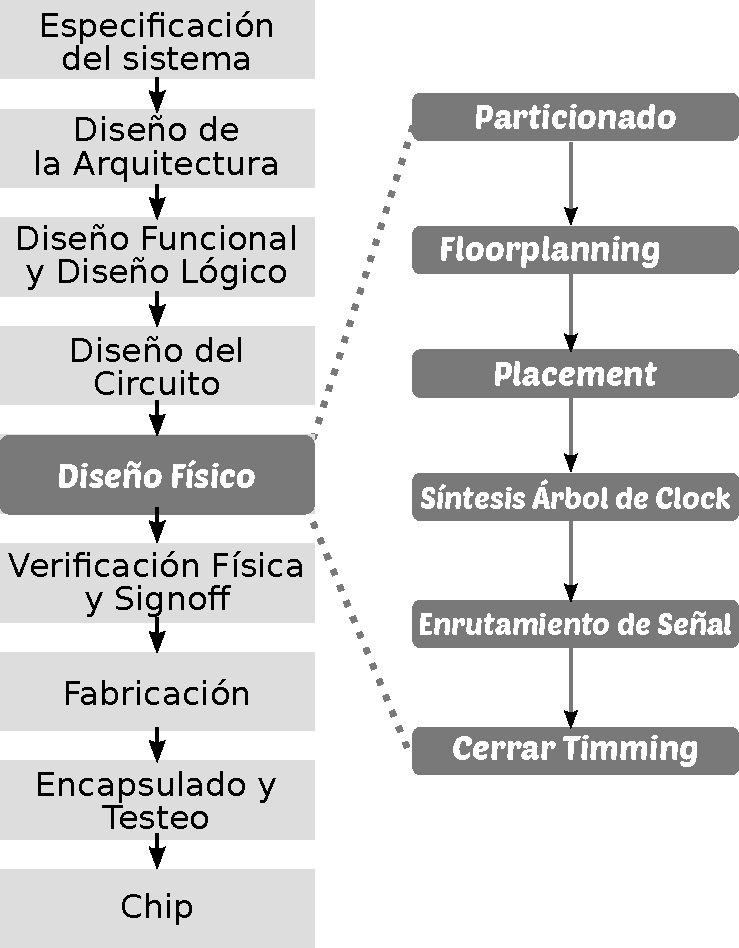
\includegraphics[scale=0.60]{figuras/DisenioFisico.pdf}
  \caption{Flujo de diseño Físico}
  \label{fig:diseñoFísico}
\end{figure}

\subsection{Etapas del diseño físico}\label{etapasDiseñoFisico}
Generalmente en un flujo de este tipo, partimos desde una descripción estructural del circuito. Esta descripción, comúnmente llamada \emph{netlist}, contiene información sobre qué bloques están presentes, y cómo estos están interconectados.



\begin{description}
\item[Particionado]
Según el tamaño del circuito, será necesario definir particiones del mismo, dividiendo el circuito en dos o mas particiones con fines de acotar la magnitud o dificultad inicial del circuito original, en partes más pequeñas de menor dificultad, si las particiones se realizan correcta e inteligentemente. 
\item[Plano general]
Luego es necesario definir un plano general del circuito (mencionado como \emph{floorplan} en la bibliografía en inglés), que impondrá condiciones físicas mínimas como el área utilizada y la disposición física de las entradas y salidas.
\item[Ubicación]
A continuación, ubicamos en este plano todos los componentes del circuito (conocido como \emph{placement} en la bibliografía en inglés), en una disposición tentativa que nos permita evaluar rápidamente la factibilidad del circuito con las condiciones impuestas por el \emph{floorplan}, por ejemplo si todos los componentes y el conexionado caben dentro del \emph{floorplan}. Depediendo de las herramientas que utilicemos, también se puede tener una estimación sobre la velocidad de las señales. 
\item[Síntesis del árbol de reloj]
Una vez que todos los elementos esten en el plano, si el circuito es secuencial, será necesario realizar una distribución de la señal del reloj para que llegue a todos los registros, de la forma más pareja (en tiempo) posible dentro de un margen de tolerancia determinado. Para ello se agregan \emph{buffers} donde sea necesario. Este proceso se conoce como \gls{cts} en la bibliografía en inglés.
\item[Conexionado]
Por último, se realiza el conexionado de todos los puertos de cada componente, utilizando las capas de metal disponible en la tecnología que se esté utilizando, un ejemplo de este conexionado se puede ver en la figura \ref{fig:routing}. Este proceso se conoce como \emph{routing} en la bibliografía en inglés.
\end{description}

En este punto, se puede realizar la mejor estimación sobre las capacidades y resistores parásitos que representan la interconexión de todo el circuito. Se encuentran los camínos críticos y se realizan las modificaciones necesarias para que el circuito cumpla con la especificaciones de retardo de propagacion máximo. Siempre en cada etapa de este proceso se puede iterar para mejorar el resultado, pero si aún así no logramos la mejora necesaria, debemos volver a iterar sobre una etapa anterior y continuar este flujo, secuencialmente.

El procesos de ubicación de los componentes e interconexionado que acabamos de describir, es muy común que se mencione como \gls{pnr}, por sus siglas en inglés.



\begin{figure}[h]
\centering
\includegraphics[scale=0.7]{figuras/Silicon_chip_3d.png}
  \caption{Representación en tres dimenciones de una celda estándar con 3 capas de metales en color arena, y una capa de silício policristalino en color ladrillo. Azul y rojo son dopado $N^+$ y $P^+$ respectivamente}
  \label{fig:routing}
\end{figure}

\section{Relevamiento, comparación y selección de las herramientas disponibles}\label{sec:herramientasDisponibles}
Para realizar las tareas que describimos en la sección \ref{etapasDiseñoFisico}, será necesario buscar una o varias herramientas de software que se ajusten a los requerimientos del diseño y la tecnología de fabricación\footnote{Se utilizará una tecnología definida por Mead y Conway\cite{mead-conway80}, conocida como  \textbf{SCMOS} (Scalable CMOS).
Esto es un conjunto de capas lógicas junto a sus reglas de diseño, que proveen un proceso casi independiente de la tecnología y dimensión, que sirve para muchos procesos CMOS disponibles a través de MOSIS.} del circuito integrado.

\paragraph{Características esperadas de las herramientas}
\begin{itemize}
\item Desarrollo activo y existencia de una comunidad de usuarios/as y desarrolladores/as que brinden soporte
\item Mayor cantidad de herramientas integradas
\item Flexibilidad para importar y exportar datos. 
\item Disponibilidad de un Kit de diseño para el proceso de la tecnología seleccionada, conocido como \gls{pdk}.
\end{itemize}

\subsection{Relevamiento}
Luego de una inspección de esas características, las herramientas candidatas que cumplen con estas características son:

\begin{description}
\item[Open Circuit Design] Proyecto de software libre que reúne en un único sitio varias herramientas independientes, mencionamos sólo algunas:  \textbf{Magic}: Layout, \gls{drc} y extracción de parásitos; \textbf{Xcircuit}: Entrada de circuitos esquemáticos; \textbf{netgen}: \gls{lvs}; \textbf{IRSIM}: simulador digital a nivel de transistor como llaves ideales, con extracción de capacidad y resistores concentrados para hacer la simulación mas realista; \textbf{Qflow}: entorno para realizar la síntesis digital con celdas estándar, utiliza Yosys\cite{Yosys}; \textbf{graywolf}: programa que realiza el \emph{placement}; \textbf{Qrouter}: programa que realiza el conexionado.

\item[Electric VLSI Design System\cite{Electric}] Es un sistema de automatización de diseño electrónico. Es un entorno integrado muy flexible que permite la descripción del circuito de varias formas (circuitos esquemáticos, \emph{netlist} VHDL y \emph{layout})). Cuenta también con herramientas para hacer \gls{drc}, \gls{lvs} y \gls{pnr}, simulación digital, visualización de formas de ondas, y un generador de \emph{pad frame}\footnote{El \emph{pad frame} es un conjunto de celdas que se ubican en el marco del \emph{die}, para conectar las señales del circuito con el exterior del chip.},entre otras herramientas.

\item[Alliance VLSI CAD System\cite{Alliance}] Alliance es un conjunto de herramientas libres, y celdas estándar para el diseño de VLSI. Incluye un compilador vhdl y un simulador, herramientas de síntesis de lógica, y herramientas de \gls{pnr} automáticas. Brinda un conjunto completo de celdas estándar CMOS escalables.

\end{description}

Es importante mencionar que existen mas herramientas disponibles (y muy útiles), pero al momento de realización de este trabajo, no forman parte de un flujo de diseño que las integre y por ello no son mencionadas aquí. 

\subsection{Comparación}
\begin{table}[h]
\begin{tabular}{@{}lll@{}}
\toprule
\textbf{Herramienta} & \multicolumn{1}{c}{\textbf{Ventajas}}                                                                                                                    & \textbf{Desventajas}                                                                                                \\ \midrule
Electric             & \multicolumn{1}{c}{Fácil instalación, acepta Python y Java como lenguajes para automatizar el diseño o implementar nuevos algoritmos de \gls{pnr}}                                                                                                                    & \begin{tabular}[c]{@{}l@{}}No incluye celdas estándar\\  caracterizadas\end{tabular}                                \\
                     & \multicolumn{1}{c}{\begin{tabular}[c]{@{}c@{}}Corre en GNU/Linux,\\  Windows, MacOS\end{tabular}}                                                        & No incluye herramienta de STA                                                                                       \\
                     & \multicolumn{1}{c}{\begin{tabular}[c]{@{}c@{}}Todas las herramientas\\  están integradas\end{tabular}}                                                   & No incluye un compilador lógico, sólo acepta netlist VHDL \\
                     & \multicolumn{1}{c}{\begin{tabular}[c]{@{}c@{}}Muchos formatos para\\ importar y exportar,\\ que nos permite utilizar \\ otras herramientas\end{tabular}} &                                                                                                                     \\
                     & \multicolumn{1}{c}{}                                                                                                                                     &                                                                                                                     \\
Open Circuit Design  & \begin{tabular}[c]{@{}l@{}}Para STA utiliza \\ celdas caracterizadas\\ para el estándar\\ abierto Liberty\end{tabular}                                   & \begin{tabular}[c]{@{}l@{}}Muchos programas para \\ instalar por separado\end{tabular}                              \\
                     &                                                                                                                                                          &                                                                                                                     \\
                     &                                                                                                                                                          &                                                                                                                     \\
                     &                                                                                                                                                          &                                                                                                                     \\
Alliance             & Algo bueno                                                                                                                                               & \begin{tabular}[c]{@{}l@{}}Las herramientas para STA\\  y conexionado no tienen\\  una licencia libre.\end{tabular} \\
                     &                                                                                                                                                          &                                                                                                                     \\
                     &                                                                                                                                                          &                                                                                                                     \\ \bottomrule
\end{tabular}
\caption{My caption}
\label{tabla:comparación}
\end{table}


%\begin{table}[h]
%\begin{tabular}{p{2cm}p{4cm}p{4cm}}
%\caption{Comparativa de las ventajas y desventajas}
%\label{tab:comparación}
%\end{table}

Resaltamos las ventajas y desventajas de cada herramienta, que nos permitirá hacer una selección en función de las necesidades del proyecto.
\subsection{Selección}
La herramienta que seleccionamos es \textbf{Electric}, ya que nos brinda una serie de ventajas comparativas, teniendo en cuenta que nuestro circuito es puramente combinacional y no demanda gran esfuerzo de \gls{pnr} a la herramienta. Podemos resumir :
\begin{itemize}
\item Fácil instalación
\item Curva de aprendizaje suave
\item Cuenta con todas las herramientas necesarias integradas
\end{itemize}
El hecho de que no cuente con un sintetizador lógico, como señalamos en la tabla \ref{tablaComparativa}, no tiene importancia para esta selección, ya que uno de los resultados del diseño digital del capítulo \ref{diseñoDigital} es un \emph{netlist} VHDL. Por la naturaleza de la solución propuesta, no deseamos que este resultado sea modificado por alguna optimización lógica, ya que rompería la interconexión original de nuestro circuito. Si quisieramos comparar nuestra implementación del circuito con la implementación automática de la operación suma, entonces tendríamos que pasar a una de las otras herramientas. Pero eso sería un trabajo de comparación de un diseño \emph{custom} con uno automático, que no era el objetivo de este proyecto. 
%Open-Source VLSI CAD Tools: A Comparative Study

\section{Selección del proceso de fabricación}\label{procesoFabricación}
%En la industria del semiconductores bajo el modelo de diseño fuera de la planta de fabricación del chip.

En este punto, es importante mencionar un aspecto de la industria de los semiconductores. En los orígenes, la industria de semicoductores estaba verticalmente integrada. Esto significaba que la misma empresa que diseñaba el producto, también diseñaba las herramientas de software y fabricaba el chip. Pero hace poco mas de 20 años, surge la separación del proceso de diseño y fabricación. Hoy en día existen empresas que se dedican sólamente a desarrollar el producto, otras que se dedican únicamente a desarrollar herramientas de software para el diseño, otras que sólamente se dedican a fabricar los diseños de otras empresas, y también persisten las empresas que realizan todo el proceso (conocidas como \gls{icms}), abriendo las puertas a otras empresas de diseño sin fábrica (conocidas como \emph{fabless}), para evitar la capacidad ociosa instalada y disminuir sus costos.
\subsection{Obleas multiproyectos}
Dentro de este esquema, existe una empresa (MOSIS) que se dedica a recolectar proyectos de diseño que están en etapa de prototipo o de bajo volumen, creando obleas multiproyecto que se envían a fabricar, dividiendo los costos por la cantidad de proyectos que incluye. De esta forma, se logra acceder a la fabricación de circuitos integrados a muy bajo costo. Tiene sus limitaciones en cuanto a tecnologías de fabricación disponibles, cantidades, y tiempo de entrega largos, pero permite que proyectos educativos, de investigación o de baja escala sean económicamente factibles. Es importante mencionar que MOSIS cuenta con un programa especial para las universidades, que permite acceder a ciertos nodos\footnote{Nodo es una forma alternativa de llamar al proceso tecnológico de fabricación que toma como segundo nombre el largo mínimo de canal de un trasistor MOS; por ejemplo: nodo de 180~\nanom ~se refiere al proceso con el cuál se puede fabricar un transistor con un mínimo de 180~\nanom~de ancho de canal.} a muy bajo costo.

Por ello, nuestras opciones serán alguna de las que MOSIS ofrece. En la tabla \ref{tab:procesosDisponibles} vemos una lista que está en constante cambio y actualización, se brinda aquí de modo ilustrativo. Para una lista actualizada visitar https://www.mosis.com/products/fab-processes.

\begin{table}[h]
\centering
\begin{tabular}{@{}lc@{}}
\toprule
Fábrica             & Proceso CMOS \\ \midrule
TSMC                & 28~nm - 180~nm             \\
Globalfoundries     & 14~nm - 180~nm             \\
IBM                 & 32~nm -  250nm            \\
ON Semi             & 0.35~um - 0.7~um           \\
Austria Micro Systems & 180~nm - 0.35~um           \\ \bottomrule
\end{tabular}
\caption{Procesos disponibles por medio de MOSIS}
\label{tab:procesosDisponibles}
\end{table}

De todas estas, elegimos TSMC 180~nm por dos razones: la primera es que cuanto mayor es la dimensión de la tecnología, más simples son las herramientas de software necesarias y más bajo es el costo de fabricación. La segunda, es que con esta tecnología se pueden realizar sistemas de gran complejidad y alta performance\footnote{Claro que cuanto más nueva es la tecnología, los circuitos digitales son más rápidos y disipan menor potencia dinámica. Pero también es cierto que mayores son los tiempos para diseñar, principalmente porque con cada nuevo nodo aparecen nuevos efectos físicos que deben ser manejados, dificultando las tareas.
}

Para dar cuenta de las capacidades de esta tecnología, vemos en la tabla \ref{tab:procesadores180nm} un conjunto de microprocesadores que la utilizaron cuando ésta era la más avanzada en su tiempo (desde el año 1999 hasta 2001) e inclusive después. Pero el verdadero sustento de que esta tecnología es actual, es que al día de hoy se continúan desarrollando varias aplicaciones, siendo una mejor opción que nodos mas nuevos, por razones económicas. Con el desarrollo de nuevas técnicas para la disminución de consumo de energía\footnote{A modo de ejemplo, ver el procesador \emph{Phoenix}, que en modo alerta consume 29.6~pW y 2.8~pJ/ciclo modo activo\cite{phoenixP}.}, la gran colección de \emph{IP}\footnote{Intelectual Property, nombre usual dado a los diseños listos para ser usados en un sistema, cuando se decide enfocar el diseño solamente en lo novedoso del producto, comprando el IP de todo lo que no diseñaremos.} analógico\footnote{Los circuitos analógicos que ya fueron diseñados y probados para una tecnología deben ser diseñados nuevamente desde cero cuando se pasa de una tecnología a otra, ya que las arquitecturas de circuitos analógicos no son escalables (como si son los digitales)} y digital que cada fábrica ofrece, las ventajas de necesitar menor poder de cálculo que para los nodos actuales (22~nm), mucha experiencia acumulada por parte de los diseñadores, se consigue un menor TTM\footnote{Time To Market (TTM), sigla utilizada para designar el tiempo que necesita un producto para ser diseñado, fabricado, testeado y puesto en producción. Dependiendo de la aplicación, este tiempo va desde meses hasta años.} con menores costos.


\begin{table}[h]
\centering
\begin{tabular}{@{}lc@{}}
\toprule
Procesador             & Año de lanzamiento \\ \midrule
Intel Coppermine E                & 1999             \\
AMD Athlon Thunderbird      & 2000             \\
Intel Celeron (Willamette)               & 2002            \\
Motorola PowerPC 7445 y 7455 (Apollo 6) & 2002           \\ \bottomrule
\end{tabular}
\caption{Procesadores fabricados en CMOS 180nm }
\label{tab:procesadores180nm}
\end{table}

MOSIS especifica los procesos disponibles que soportan las reglas escalables en su documento \emph{\textbf{Design Rules. MOSIS Scalable CMOS (SCMOS), Revision 8.00.}}, en el cuál encontramos que para 180~nm sólo podemos elegir a la fábrica TSMC.

Además, podemos optar entre las reglas \textbf{SCN6M\_SUBM} y las \textbf{SCN6M\_DEEP}. Decidimos utilizar la segunda, ya que tiene un valor de $\lambda$ menor, lo cual significa un tamaño de transistor resultado más óptimo.

El proceso nos ofrece 6 capas de metal (aluminio) para la interconexión, 1 capa de silicio policristalino (\emph{poly}) para crear la compuerta y también para la interconexión de las mismas (distancias cortas sólamente, por su mayor resistividad que el cobre), con 2 tipos de óxidos para crear el aislante de las compuertas, los que pueden ser alimentados con tensión máxima de 1,8V, y los que pueden ser alimentados con 3,3V (pensados principalmente como transistores para los circuitos de entrada y salida del chip). MOSIS denomina a las reglas de diseño que utilizaremos para esta tecnología como SCN6M\_DEEP, que significa: 
\begin{itemize}
\item S: Escalable
\item C: Tecnología de fabricación CMOS
\item N: Pozo N.
\item 6M: 6 metales y un conductor policristalino (\emph{poly}) para crear las compuertas.
\item DEEP: Reglas \emph{deep submicron}.
\end{itemize}
Las reglas escalables se crearon originalmente para tecnologías desde 3um hasta 1um. Cuando aparecieron tecnologías nuevas, se hicieron modificaciones a las reglas para ajustarse a las nuevas posibilidades. Entonces se crearon primero las reglas \emph{submicron}, y luego las \emph{deep submicron}

Una vez definido la herramienta de diseño (\textbf{Electric}) y el proceso de fabricación a utilizar (TSMC 180~nm), definimos la variable $\lambda$, que es la unidad que utilizará nuestro software para las dimensiones físicas. \textbf{Electric} define a $\lambda$ como la mitad del largo de canal mínimo para la tecnología que se está utilizando. En nuestro caso, el largo de canal mínimo es de 180~nm (de allí viene la designación del nombre), por lo tanto $\lambda $ es de 90~\nanom.  


\subsection{\emph{Corners} de simulación}

Debido a las variaciones propias del proceso de fabricación, obtendremos variaciones en las dimensiones físicas de los transistores y capas de metales. Por ello podemos esperar que el chip que probemos en el laboratorio luego de la fabricación contenga transistores que pueden ser lentos, típicos o rápidos, y que las interconexiones sean mas o menos capacitivas y resistivas. Generalmente todos los transistores e interconexiones dentro del chip seran de un sólo tipo. Por ello, el fabricante nos brinda modelos de simulación para los distintos casos de transistores que podemos esperar; y lo mismo con las capas de metal, nos brinda unas tablas que representan las distintas resistividades y capacidades parásitas que podemos esperar.
Existe también la variación de tensión que puede tener la alimentación del circuito que vayamos a estudiar, ya que el diseño de la malla interna de alimentación se calcula con un margen de tolerancia de caída de tensión máxima. Por lo tanto podemos esperar que la alimentación de nuestro circuito sea de un \%10 menor que la tensión nominal, por ejemplo.
Por último, la temperatura ambiente impacta fuertemente en las características eléctricas del circuito integrado.

Por todo esto que mencionamos, se definen casos de simulación para contemplar las peores y mejores condiciones que podemos esperar. Este conjunto de casos se denominan \emph{corners} de simulación. Por ejemplo, la peor condición para la performance 
es una temperatura de 0 grados, transistores lentos, capacidades mayores que la media y la tensión de alimentación un \%10 menos que la nominal. Pero la peor condición desde el punto de vista del consumo de energía es 80 grados de temperatura ambiente, transistores rápidos, tensión nominal y capacidades mayores que la media.
Como conclusión, debemos tener en cuenta las peores y mejores condiciones para realizar las simulaciones correspondientes, si esperamos que la simulación nos sirva para diseñar y lograr que la mayoría de los chips de un lote fabricado cumpla con las especificaciones de diseño. 

En nuestro caso, utilizaremos un único modelo de transistores y capacidades y resistores parásitos que MOSIS brinda en su sitio web a modo de ejemplo del proceso de fabricación, ya que para obtener los \emph{corners} de simulación es necesario contratar el servicio previamente. Tomamos ese modelo como el caso típico, y todas las simulaciones se hacen con 27 grados de temperatura ambiente y tensión de alimentación nominal (1.8~V).

\section{Selección de las Celdas estándar}\label{celdasEstandars}
El resultado de la síntesis que realizamos en el capítulo \ref{diseñoDigital} es un \emph{netlist} VHDL que contiene sólo compuertas lógicas. Estas son compuertas lógicas abstractas, es decir que nuestro circuito fué mapeado a un conjunto finito de funciones logicas como las \verb.and., \verb.or., \verb.xor., \verb.xnor., etc.

Ahora es necesario mapear estas funciones lógicas a compuertas lógicas reales, que serán tambien un conjunto finito de compuertas, pero con dimensiones físicas definidas, y con una caracterización de su funcionamiento real. Estas compuertas lógicas se denominan celdas estándar, que sirven específicamente para la tecnología de fabricación que hayamos definido usar. Por cada función lógica existen distintas versiones de la misma función, pero con distintas características eléctricas. Mostramos en la figura \ref{fig:map-xnor} un ejemplo de una celda estándar que implementa la función lógica \verb.xnor.

%Caraterización de las celdas: Se realizan simulaciones analógicas de un netlist de estas celdas, donde variando paramétricamente la carga (capacitiva) de salida y el tiempo de crecida y caída ($t_r$ y $t_f$) de la entrada, se obtiene el retardo de propagación, tiempo de crecida y de bajada de la salida y la disipación de potencia.


% Dibujo de una XOR en netlist mapeado a una XOR en layout.

\begin{figure}[h]
\centering
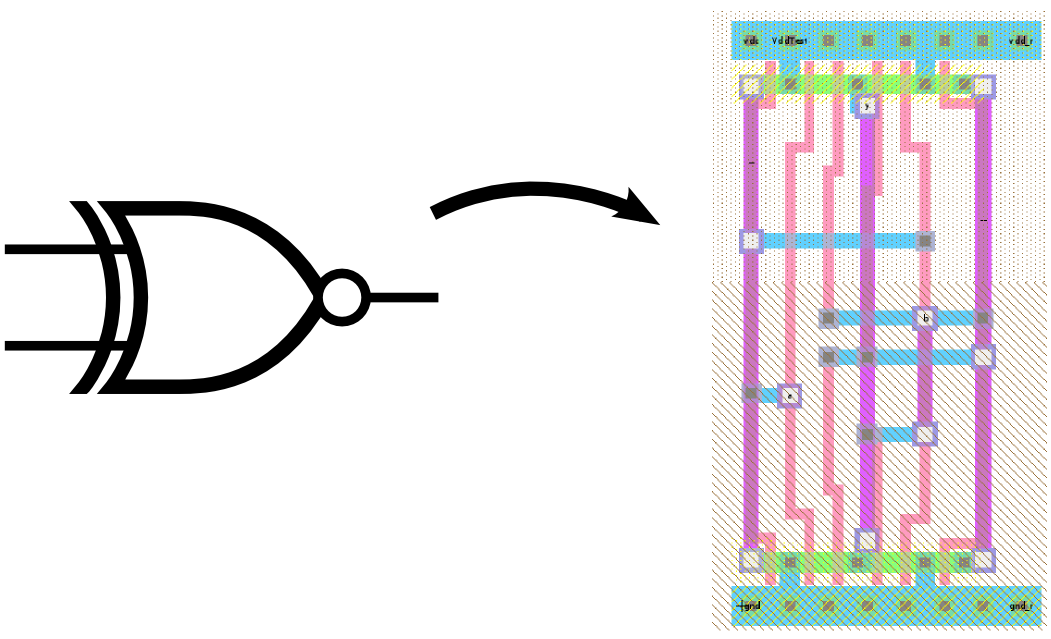
\includegraphics[scale=0.7]{figuras/map-xnor.png}
  \caption{Mapeo de una función lógica a una celda estándar}
  \label{fig:map-xnor}
\end{figure}

Es común elegir las celdas estándar según el tipo de aplicación a desarrollar. Existen celdas estandar que fueron diseñadas para bajo consumo, o alta velocidad, o de mínima área. También existe la posibilidad de diseñar celdas que busquen la mejor relación velocidad-consumo-area que puedan ser utilizadas en muchas aplicaciones. En circuitos integrados para sistemas alimentados a batería se intentará utilizar las celdas de menor consumo y evitar siempre que sea posible las de mayor velocidad, en función del presupuesto de potencia disponible para el mismo.

En nuestro caso, aprovechando que la suma se realiza con apenas 3 compuertas: \verb.and., \verb.or., \verb.xor., podemos construir nuestro propio conjunto de celdas. Como punto de partida, utilizamos celdas que fueron realizadas para un estudio sobre circuitos digitales operando por debajo de la región de inversión débil\cite{subthresholdArith}.
 %Una referencia al Rabaey es necesaria? 
\subsection{Características}
Estas celdas están correctamente dimensionadas para lograr el apilamiento en filas y columnas, y una grilla de interconexionado amplia, que nos evitará problemas de este tipo. Para nuestros objetivos, modificamos las dimensiones de los transistores de canal P, para lograr un tiempo de crecida y bajada más simétricos, y así mejorar la velocidad. Resumimos las características de nuestras celdas estándar:


\begin{description}
\item[Altura] 128 $\lambda$\footnote{En la bibliografía en ingles se denomina \emph{pitch}}, es la distancia desde el riel de Vdd hasta Vss, lo cual permite el ruteo horizontal de 16 pistas de metal por encima de las celdas, con metal 3 hasta capas superiories, como vemos en la figura \ref{fig:pitchCeldaEstandar}.  
\item[Ancho del riel de alimentación] 8 $\lambda$
\item[Tamaño de los transistores] Transistores \verb.n.: largo y ancho mínimo ($L_n = 2 \lambda$, $W_n =4 \lambda$, $\frac{W_n}{L_n}=2$). Transistores \verb.p.: Largo mínimo. Dos versiones, una de ancho mínimo con $\frac{W_p}{L_p}=2$ y otra de mayor fuerza $\frac{W_p}{L_p}=4$, a la que le agregamos \verb._1x. al final del nombre. 
\item[Disposición de los pines] Se ubican siempre en la intersección de las pistas horizontales y verticales, que tienen una separación de $8 \lambda$, ver figura \ref{fig:pitchCeldaEstandar}.
\item[Conexión a bulk] Todas las celdas tienen conexión a bulk cada $8\lambda$ para evitar el problema conocido como \emph{latch up} que surge a causa de malas conexiones entre el \emph{bulk} y la alimentación.
\end{description}


Otra característica de estas celdas es la distancia entre el riel de VSS hasta el riel de VDD. Esta distancia es de 128 $\lambda$, lo cual permite el ruteo horizontal de 16 pistas de metal por encima de las celdas, con metal 3 hasta capas superiories, como podemos ver en la figura \ref{fig:pitchCeldaEstandar}.  

 \begin{figure}[h]
\centering
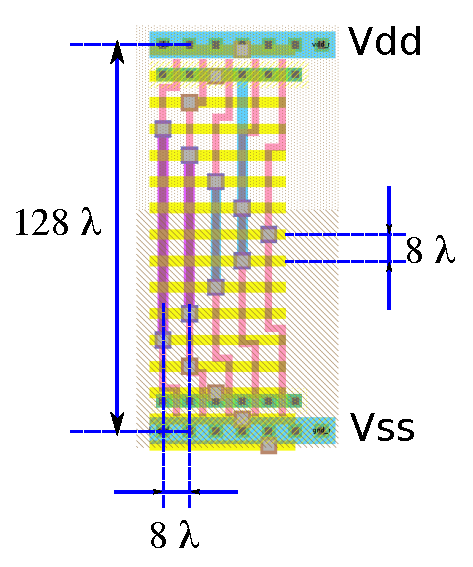
\includegraphics[scale=.7]{figuras/CeldEstandarAlto.eps}
  \caption{Grilla de interconexionado y riel de alimentación de las celdas estándar de $128 \lambda$. Por encima de cada celda, pueden pasar 16 pistas horizontales que la herramienta de conexionado tendrá a disposición, a partir del metal 3 para arriba. Notar la separación de $8~ \lambda$ para todas las pistas horizontales, y $8~\lambda$ para las verticales también. Sólo en la intersección de las pistas puede ubicarse los pines de entrada/salida de la celda, así como los contactos a \emph{bulk}.}
  \label{fig:pitchCeldaEstandar}
\end{figure}

\begin{figure}
        \centering
        \begin{subfigure}[b]{0.15\textwidth}
                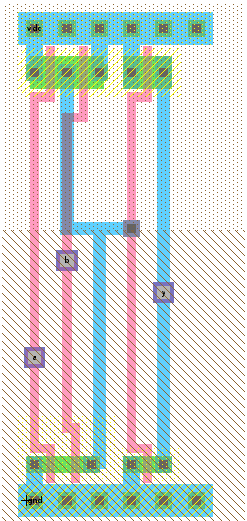
\includegraphics[width=1.075\textwidth]{figuras/and2_1x.png}
                \caption{and2\_1x}
                \label{fig:gull}
        \end{subfigure}\quad
        ~ %add desired spacing between images, e. g. ~, \quad, \qquad, \hfill etc.
          %(or a blank line to force the subfigure onto a new line)
        \begin{subfigure}[b]{0.15\textwidth}
                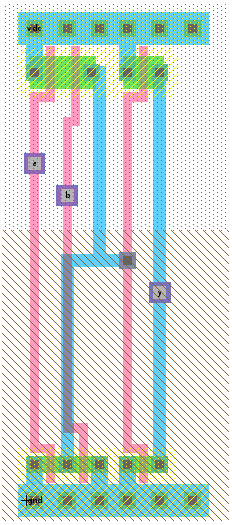
\includegraphics[width=1\textwidth]{figuras/or2_1x.png}
                \caption{or2\_1x}
                \label{fig:tiger}
        \end{subfigure} 
        ~ %add desired spacing between images, e. g. ~, \quad, \qquad, \hfill etc.
          %(or a blank line to force the subfigure onto a new line)
        \begin{subfigure}[b]{0.15\textwidth}
                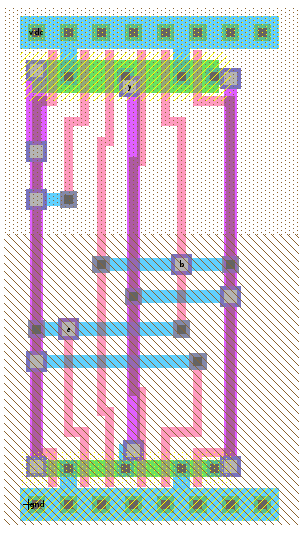
\includegraphics[width=1.31\textwidth]{figuras/xor2_1x.png}
                \caption{xor\_1x}
                \label{fig:mouse}
        \end{subfigure}\qquad
        \begin{subfigure}[b]{0.15\textwidth}
                \includegraphics[width=0.845\textwidth]{figuras/id_1x_.png}
                \caption{buffer}
                \label{fig:mouse}
        \end{subfigure}
        \caption{Conjunto de celdas estándar}\label{fig:animals}
\end{figure}






%http://cmosedu.com/cmos1/electric/electric.htm
% “Tiny-Chip” padframes [1.5 mm x 1.5 mm]

\section{Ubicación y Cableado (\emph{Place \& Route})}
Partimos desde la descripción estructural\footnote{El resultado de la síntesis hecha con \textbf{lava} es un \emph{netlist} VHDL a nivel de compuerta, listo para ser usado por una herramienta de \gls{pnr}.} que producimos en el capítulo \ref{diseñoDigital}. De \emph{Electric} usaremos la herramienta llamada \textbf{\emph{Silicon Compiler}}, que se encarga de ubicar y conectar las celdas según el \emph{netlist} VHDL.

\subsection{Modificación al código fuente de la herramienta de síntesis lógica}

La herramienta \textbf{\emph{Silicon Compiler}} requiere que el \emph{netlist} VHDL sea modificado levemente:
\begin{enumerate}
%\item Reemplazar los nombres de las instancias de las celdas estándar que seleccionamos en la sección \ref{celdasEstandars} y \emph{Electric} utilizará.
\item\label{celdas} Es necesario agregar las celdas estándar como componente en la porción declarativa de la arquitectura de la entidad  en VHDL, que serán utilizadas instanciadas en el circuito.
\item\label{caracteres} Los nombres no pueden usar los símbolos [ y ], por lo cual es necesario eliminarlos.
\end{enumerate} 
 
Modificamos el código del programa de \textbf{lava} llamado \verb|VhdlNew.hs|, encargado de crear el \emph{netlist} VHDL para realizar (\ref{celdas}), y para lograr (\ref{caracteres}) agregamos una línea para que lance un pequeño programa escrito en \textbf{perl} que mostramos en el apéndice \ref{scriptPerl}. Luego de esta modificación, cuando realizamos la síntesis lógica descripta en el capítulo \ref{diseñoDigital}, el \emp{netlist} VHDL obtenido ya puede ser utilizado por \textbf{\emph{Silicon Compiler}}.



\subsection{Configuración de la herramienta de \gls{pnr}}
En la figura \ref{fig:SCconf} vemos la configuración necesaria para hacer el \gls{pnr} con nuestras celdas estándar. La configuración se realiza para ajustar la herramienta a las reglas de \gls(drc) y las dimensiones de nuestra celdas estándar. La variable de ajuste para modificar el \emph{floorplan} es el parámetro \emph{Number of rows of cells}. Según la cantidad de filas que asignemos, será el resultado obtenido para cada circuito. 


% Configuración del Silicon Compiler
\begin{figure}[h]
\centering
\includegraphics[scale=0.65]{figuras/SCconf.png}
  \caption{Configuración del Silicon Compiler}
  \label{fig:SCconf}
\end{figure}


\subsection{Distintas alternativas y resultados}
La regla de oro para todo \emph{layout} es que sea lo más cuadrado posible, ya que de esta forma es más eficiente el uso del área cuando integramos nuestro circuito con otros de mayor jerarquía. La métrica de selección del resultado será el área que ocupe nuestro circuito y la relación entre sus lados: cuanto más pequeño\footnote{El área es una métrica de calidad del circuito, según lo planteamos en el capítulo \ref{chap:especificaciones}.} y cuadrado mejor. En las tablas \ref{tab:rippleCarry}, \ref{tab:sklansky} y \ref{tab:brent-kung} vemos los resultados para todos los sumadores analizados, con 3 tamaños distintos y para diferentes alternativas de \emph{floorplan}, variando el parámetro \textbf{\emph{Number of rows of cells}}.

En la figura \ref{fig:diseños} presentamos todos los \emph{layout} seleccionados con el criterio recién mencionado. Resumimos con este gráfico el resultado de \gls{pnr} de cada arquitectura para 3 tamaños de sumandos distintos.
\begin{table}[h]
\centering
\resizebox{\textwidth}{!}{%
\begin{tabular}{@{}cccccccccc@{}}
\toprule
\multicolumn{1}{l}{\textbf{Ripple Carry}} & \multicolumn{3}{c}{8}    & \multicolumn{3}{c}{16}      & \multicolumn{3}{c}{32}      \\ \midrule
filas                                     & 3      & 4      & 5      & 5       & 6       & 7       & 8       & 7       & 6       \\
ancho                                     & 1297   & 966    & 843    & 1562    & 1350    & 1142    & 1881    & 2169    & 2581    \\
alto                                      & 665    & 839    & 958    & 1227    & 1196    & 1600    & 2000    & 1850    & 1360    \\
área                                      & 862505 & 810474 & 807594 & 1916574 & 1614600 & 1827200 & 3762000 & 4012650 & 3510160 \\
ancho/alto                                & 0,51   & 0,87   & 1,14   & 0,79    & 0,89    & 1,40    & 1,06    & 0,85    & 0,53    \\ \bottomrule
\end{tabular}
}
\caption{Ubicación y conexionado para Ripple carry en 3 tamaños: 8, 16 y 32 bits}
\label{tab:rippleCarry}
\end{table}

\begin{table}[h]
\centering
\resizebox{\textwidth}{!}{%
\begin{tabular}{@{}ccccccccccc@{}}
\toprule
\textbf{Sklansky} & \multicolumn{3}{c}{8}       & \multicolumn{4}{c}{16}                & \multicolumn{3}{c}{32}      \\ \midrule
filas              & 3       & 4       & 5       & 4       & 5       & 6       & 7       & 6       & 7       & 8       \\
ancho              & 1516    & 1167    & 954     & 3538    & 2042    & 1825    & 1536    & 3678    & 3229    & 2860    \\
alto               & 810     & 973     & 1252    & 1345    & 1581    & 1878    & 2063    & 2639    & 2695    & 3072    \\
área               & 1227960 & 1135491 & 1194408 & 4758610 & 3228402 & 3427350 & 3168768 & 9706242 & 8702155 & 8785920 \\
ancho/alto         & 0,53    & 0,83    & 1,31    & 0,38    & 0,77    & 1,03    & 1,34    & 0,72    & 0,83    & 1,07    \\ \bottomrule
\end{tabular}
}
\caption{Ubicación y conexionado para Skalanksy en 3 tamaños: 8, 16 y 32 bits}
\label{tab:sklansky}
\end{table}

\begin{table}[h]
\centering
\resizebox{\textwidth}{!}{%
\begin{tabular}{@{}cccccccccccc@{}}
\toprule
\textbf{Brent-Kung} & \multicolumn{3}{c}{8}      & \multicolumn{4}{c}{16}                & \multicolumn{4}{c}{32}                \\ \midrule
filas               & 3       & 4      & 5       & 4       & 5       & 6       & 7       & 6       & 7       & 8       & 9       \\
ancho               & 1386    & 1090   & 945     & 2268    & 1757    & 1545    & 1429    & 3196    & 1983    & 2569    & 2424    \\
alto                & 746     & 910    & 1199    & 1255    & 1436    & 1540    & 1959    & 2024    & 2871    & 2927    & 2882    \\
área                & 1033956 & 991900 & 1133055 & 2846340 & 2523052 & 2379300 & 2799411 & 6468704 & 5693193 & 7519463 & 6985968 \\
ancho/alto          & 0,54    & 0,83   & 1,27    & 0,55    & 0,82    & 1,00    & 1,37    & 0,63    & 1,45    & 1,14    & 1,19    \\ \bottomrule
\end{tabular}
}
\caption{Ubicación y conexionado para Brent-Kung en 3 tamaños: 8, 16 y 32 bits}
\label{tab:brent-kung}
\end{table}


\begin{figure}
\centering
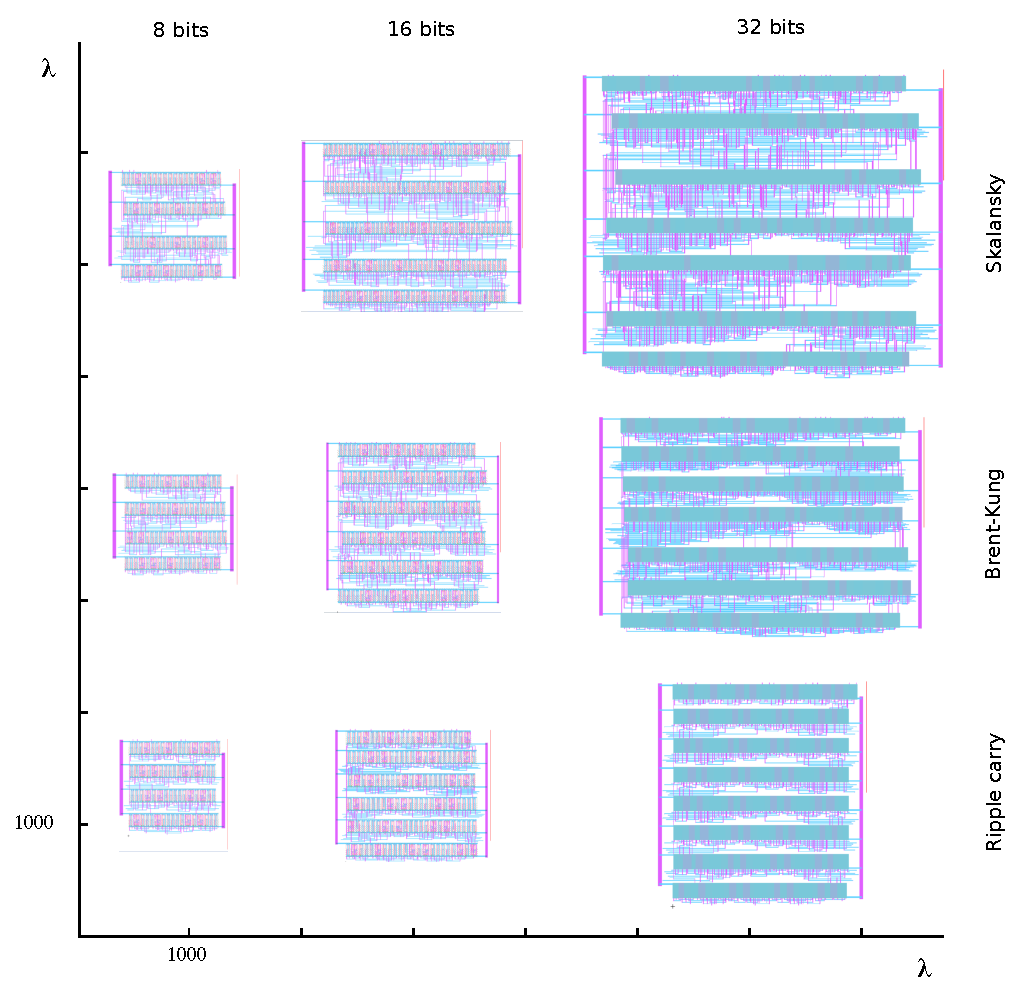
\includegraphics[scale=1]{figuras/PnR9disenos.eps}
  \caption{Tres arquitecturas y tres tamaños de sumandos distintos. Los circuitos están en escala, la unidad de los dos ejes es $\lambda=90~\nanom$}
  \label{fig:diseños}
\end{figure}

\section{Comparación de las distintas arquitecturas}

\subsection{Simulación post \emph{layout} para calcular performance y potencia}
Para realizar la comparación, necesitamos simular nuestros circuitos luego de hacer una extracción del \emph{layout} del circuito, para obtener también las capacidades y resistores párasitos del mismo. A esta simulación se le suele denominar, simulación post \emph{layout}.

\subsubsection{Extracción del circuitos, las dimensiones físicas de los transisitores y elementos parásitos}

Para realizar una simulación que sea la mejor estimación de la performance y potencia, es necesario realizar una extracción del circuito a partir del \emph{layout}, y para eso es necesario configurar \textbf{Electric} de la siguiente forma:

\begin{itemize}
\item Parámetros del modelo de transistor: Cargar los modelo de transistores de la tecnología que estamos usando (TSMC 180~nm). Este es un archivo que nos brinda MOSIS, del cual la primera parte nosotros debemos comentar (ya que es toda la información propia de la tecnología y no solamente la específica para el simulador), y renombramos como {\footnotesize\verb#tsmc180nm.model#}. También es necesario realizar los siguientes cambios al archivo:\\
\begin{footnotesize}\verb#.MODEL CMOSN NMOS#\end{footnotesize} cambiar por \begin{footnotesize}\verb#.MODEL N NMOS# \\
\verb#.MODEL CMOSP PMOS#\end{footnotesize} cambiar por \begin{footnotesize}\verb#.MODEL P PMOS# \end{footnotesize} \\
Luego de esos cambios, cargar el archivo en:\\
\begin{footnotesize}\verb.File -> Preferences -> Tools -> Spice/CDL -> Use Header cards from file:.\end{footnotesize}
	\item Del archivo recién mencionado obtenemos la resistividad de los metales, el \emph{poly}, el sustrato y el silicio dopado $N^+$ y $P^+$. También obtenemos la capacidad entre cada capa de material y el resto de las capas. Esta información la utilizamos para configurar \textbf{Electric} en: \\
\begin{footnotesize}\verb.File -> Preferences -> Tools -> Parasitic. \end{footnotesize}
\item Extracción de parásitos: Para realizar la extracción de las capacidades y resistores parásitos de las interconexiones: \\
\begin{footnotesize}\verb.File -> Preferences -> Tools -> Spice/CDL -> Parasitics: Conservative RC. \end{footnotesize}
\item Seleccionar el formato (lenguaje) del \emph{netlist spice} del simulador que utilizaremos: Las opciones son: \textbf{Spice 2, Spice 3, HSpice, PSpice, Gnucap, SmartSpice,  Spice Opus, Xyce, HSpice for Assura, HSpice for Calibre}. De los cuales, sólo 3 opciones tienen licencias calificadas como software libre: \textbf{Spice 3, Gnucap} y \textbf{Xyce}. \textbf{Spice 3} hace referencia a la versión \textbf{Spice3f5} del estándar de facto para las simulaciones de circuitos analógicos, en general todos los programas pueden leer un \emph{netlist} en ese formato.
\end{itemize}


\begin{figure}
%\vspace{-5pt}
  \centering
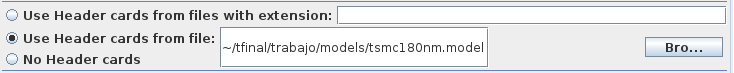
\includegraphics[scale=.5]{figuras/gnucapElectric3.png}
  \caption{Configuración de Electric para la extracción del circuito y simulación en un motor tipo Spice.}
\label{fig:gnucapElectric}
%\vspace{-10pt}
\end{figure}



\subsubsection{Motores de simulación analógica}

De la lista de opciones que nos brinda \textbf{Electric}, hacemos una selección y breve reseña de los simuladores de circuitos que tienen licencia calificadas como software libre:


\begin{description}
\item[Gnucap] Simulador de circuitos analógicos y señal mixta, está diseñado para reemplazar Spice, pero con ventajas técnicas significantes. Más rápido e igual de preciso, diseñado para alta flexibilidad por medio de un sistema de \emph{plugins}, permite elegir qué algoritmos utilizará el \emph{solver}, relación de compromiso entre precisión y velocidad controlado por el usuario, totalmente interactivo por medio de \emph{scripting}. Puede leer \emph{netlists} en formato tradicional \textbf{Spice 3}, \textbf{Spectre}\footnote{Motor de simulación de Cadence.} y  \emph{netlist} Verilog.

\item[Ngspice] Simulador de circuitos de señal mixta. Se basa en tres paquetes de software libre: Spice3f5, Cider1b1 y Xpice. Implementa muchas mejoras y cuenta con una comunidad de desarrolladores y usuarios que dan soporte y corrección de \emph{bugs}. Fué ampliamente incorporado en otros entornos de simulación de circuitos, por ser la continuación con licencia libre del Spice3f5.

\item[Xyce] Simulador de circuitos con compatibilidad Spice, implementa mejoras para lograr simulaciones de millones de transistores con la misma precisión. Implementa alto nivel de paralelismo, \emph{solvers} iterativos mejorados y simula efectos de radiación (corriente de fotones y destrucción de neutrones).
\end{description}

\subsubsection{Selección del simulador}
Desde el punto de vista de la instalación de las herramientas, Ngspice y Xcye son más complicadas con respecto a Gnucap. Las características distintivas de estos dos proyectos no son necesarias para las simulaciones de nuestros diseños en particular. Por ello decidimos utilizar \textbf{Gnucap} ya que es de múy fácil instalación en el sistema operativo que estamos utilizando (Debian "Wheezy"). 

Ahora que ya tenemos seleccionado el simulador y configurada la herramienta para realizar la extracción, lo primero que simularemos es un oscilador anillo de 31 etapas, para dar cuenta de lo que logramos con nuestro flujo de herramientas (\textbf{Electric} + \textbf{Gnucap}), en comparación con lo que MOSIS brinda de esa prueba:

\begin{footnotesize}
\begin{verbatim}
 Ring Oscillator Freq.                                   
  DIV1024 (31-stg,1.8V)               377.13  MHz        
 Ring Oscillator Power                                   
  DIV1024 (31-stg,1.8V)                 0.02  uW/MHz/gate
\end{verbatim}
\end{footnotesize}

\subsubsection{Simulación de un oscilador anillo}
Realizamos el layout del oscilador anillo de 31 etapas que mostramos en la figura \ref{fig:lay_31etapas}, y realizamos la simulación de régimen transitorio. Para ver la frecuencia de oscilación, guardamos los datos de la tensión de una salida de uno de los inversores, y para calcular la potencia, guardamos la corriente que sale de la fuente de alimentación. Nuestros resultados son:

\begin{table}[h]
\centering
\begin{tabular}{@{}lcc@{}}
\toprule
Circuito	&	Frecuencia de oscilación	&	Potencia \\ \midrule
Oscilador anillo de 31 etapas               & 325 MHz	& 0.026 uW/MHz/compuerta   \\ \bottomrule
\end{tabular}
\caption{Simulación post \emph{layout} del oscilador anillo de 31 etapas}
\label{tab:RO31}
\end{table}

Justificamos la diferencia entre nuestros resultados y los datos brindados por el fabricante en que no existe un detalle de la prueba de caracterizaciónn de la tecnología de fabricación. Es decir, no brinda las dimensiones físicas del inveror utilizado, cómo fué interconectado, etc, lo cual impacta fuertemente en la performance y potencia.


\begin{figure}
%\vspace{-5pt}
  \centering
\includegraphics[scale=.35]{figuras/lay_31etapas.png}
  \caption{Oscilador anillo de 31 etapas}
\label{fig:lay_31etapas}
%\vspace{-10pt}
\end{figure}

\subsection{Medición de la performance en un sumador}\label{sec:performance}
Siguiendo lo que definimos en el capítulo \ref{chap:especificaciones} para la performance, ahora seremos más específicos para los sumadores y definiremos las condiciones que nos permiten medir correctamente el tiempo de propagacion $t_p$ del camino crítico. Realizaremos dos simulaciones de régimen transitorio para que el estado de las entradas cambie de forma tal que exite el camino crítico. Una simulación para encontrar $t_{pHL}$ y otra para $t_{pLH}$.

Para eso necesitamos generar cambios de estados que generen acarreo en todos los bits, ya que el bit mas significativo de la suma y el acarreo de salida, dependen de los acarreos del bit anterior. Si logramos que desde el bit menos significativo se propague hasta el más significativo, estamos exitando el camino crítico para que se propague la señal desde los bits menos significativos a los más significativos. Esto se puede lograr con las siguientes 2 transiciones (ejemplo para un sumador de 8 bits):

\begin{equation}\label{eq:tfhl}
(A_0,B_0) \to (A_1,B_1) = (\textrm{0x00}, \textrm{0xFF}) \to (\textrm{0x01},\textrm{0xFF})
\end{equation}
\begin{equation}\label{eq:tflh}
(A_1,B_1) \to (A_0,B_0) = (\textrm{0x01},\textrm{0xFF}) \to (\textrm{0x00}, \textrm{0xFF})
\end{equation}

Como el estado final de una transición es el estado inicial de la otra, y viceversa, podemos realizar estas dos mediciones con una sóla simulación de régimen transitorio que cíclicamente pase de un estado al otro. Eso es lo que mostramos en la figura \ref{fig:sim_rca8}, que utilizamos para encontrar el camino crítico. Vemos que la señal \verb.s7. es la más lenta, y que la transición \ref{eq:tfhl} nos sirve para calcular $t_{pHL}$. La transición \ref{eq:tflh} nos permite calcular $t_{pLH}.
	 	

\begin{figure}
%\vspace{-5pt}
  \centering
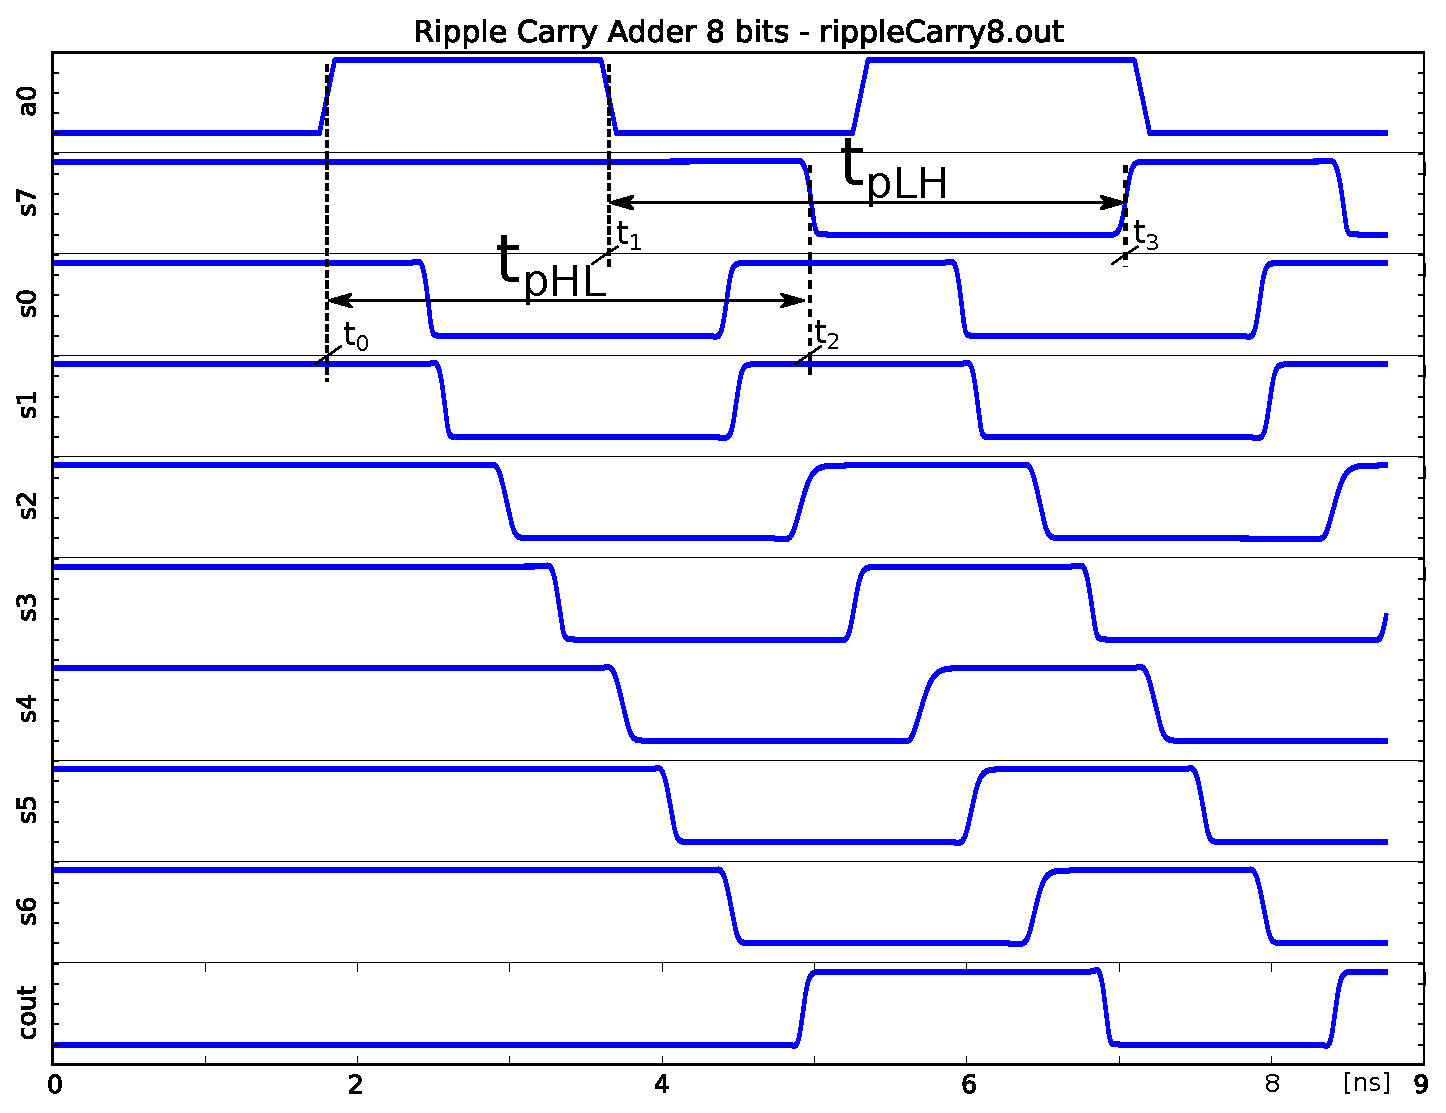
\includegraphics[scale=.64]{figuras/sim_rca8bits_.eps}
  \caption{Simulación de régimen transitorio del circuito Ripple Carry 8 bits. De los vectores de entradas, sólo mostramos el bit menos significativo de la entrada A, porque es el único que cambia. Las señales de salidas están ordenadas para mostrar la más lenta cerca de la entrada y poder calcular el retardo.}
\label{fig:sim_rca8}
%\vspace{-10pt}
\end{figure}

\begin{figure}
%\vspace{-5pt}
  \centering
 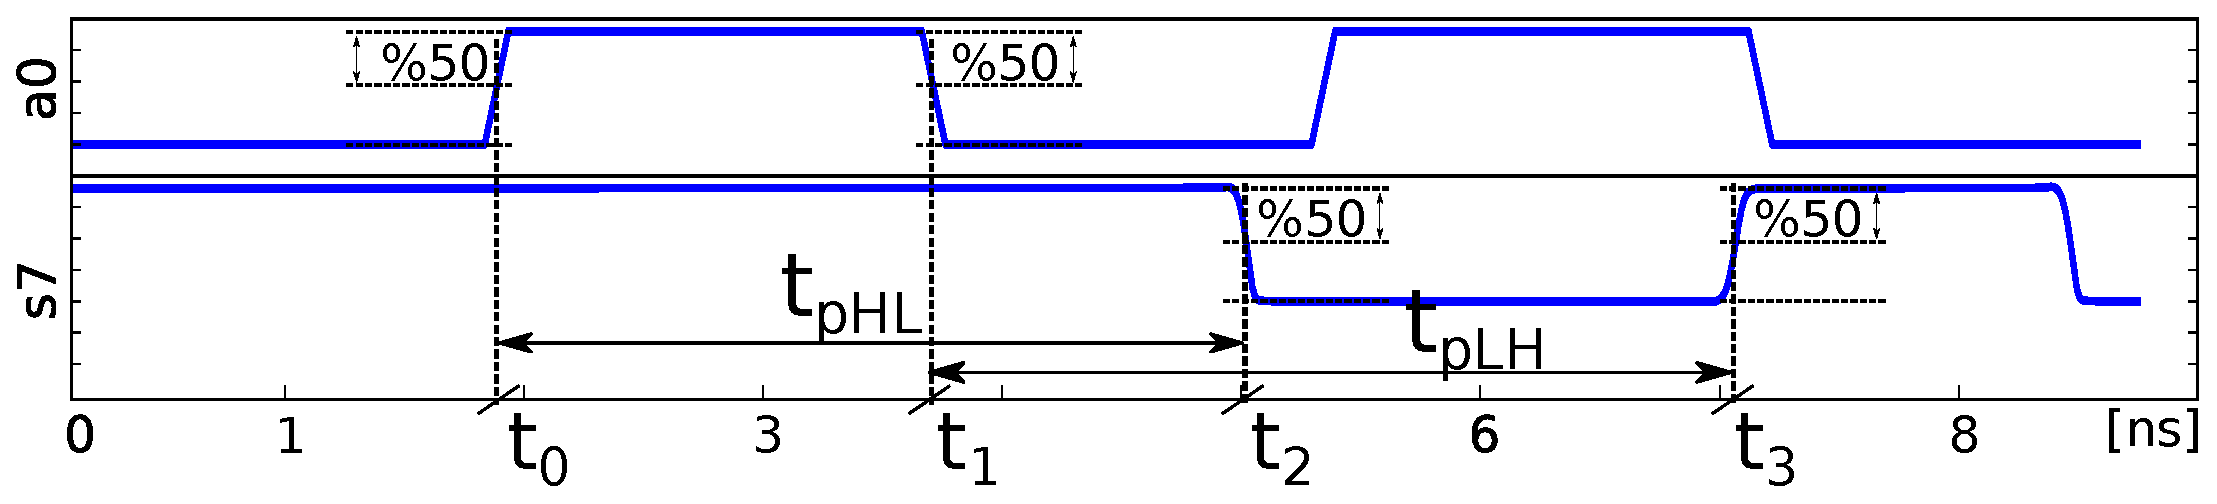
\includegraphics[scale=.45]{figuras/rca8bits_zoom.eps}
  \caption{Simulación de régimen transitorio del circuito Ripple Carry 8 bits. Para calcular $t_{pHL}$ y $t_{pLH}$ lo hacemos sobre la señal más lenta del circuito, que en este caso es el bit más significativo de la suma }
\label{fig:sim_rca8_zoom} 
%\vspace{-10pt}
\end{figure}
De la figura \ref{fig:sim_rca8_zoom} extraemos los datos para realizar la medición del $t_p$ del sumador de \textbf{ripple carry de 8 bits}:

%t_0 = 1.8
%t_1 = 3.64
%4.96
%7.05

$$t_{pHL} = t_2 - t_0 = 5.01~\ns - 1.8~\ns = 3.21~\ns$$
$$t_{pLH} = t_3 - t_1 = 7.05~\ns - 3.61~ns = 3.44~\ns$$
$$t_p = \frac{(t_{pHL} + t_{pLH} )}{2} = 3.325~\ns$$



\subsection{Medición de la potencia en un sumador}\label{sec:potencia}

La actividad de una señal afecta tanto a la potencia estática de un circuito CMOS como a la potencia dinámica. La potencia estática depende del estado de la señal, y la potencia dinámica depende de la tasa de cambio de los pines en cada celda estándar. Nuestra simulación para la potencia comparte los mismos vectores de entrada que el de performance, ya que con estos vectores generamos la mayor actividad posible en los pines de salida. En la figura \ref{fig:sim_rca8_pow} podemos ver las formas de onda de la exitación y la corriente instantánea que sale de la fuente de alimentación. Para obtener el valor de la potencia del circuito, aplicamos la ecuación \ref{eq:pv}, que lo realizamos directamente con el simulador, obteniendo una potencia promedio total de:
$$P_{av} = \frac{1}{\mathrm{{t_f - t_i}}}\int\limits_{t_i}^{t_f} p(t)dt = \mathrm{\frac{1.8~V}{3.5~\ns}}\int\limits_{3.5~\ns}^{7~\ns} i_{\mathrm{fuente}}(t)\mathrm{d}t $$
$$P_{av} = -838.269~\mu\textrm{W}$$

\begin{figure}
%\vspace{-5pt}
  \centering
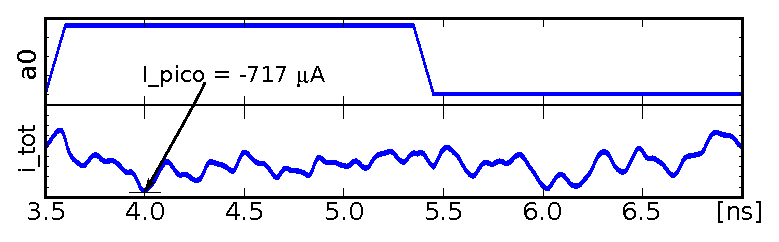
\includegraphics[scale=1.1]{figuras/rca8bits_power.eps}
  \caption{Simulación de régimen transitorio del circuito Ripple Carry 8 bits. Mostramos la corriente instantánea a través de la fuente de alimentación, el valor negativo se debe a que la corriente sale de la fuente. }
\label{fig:sim_rca8_pow}
%\vspace{-10pt}
\end{figure}
El período de integración que elegimos está determinado por el $t_p$ del circuito, lo que físicamente quiere decir: Medimos la potencia del circuito cuando está funcionando a la mayor velocidad posible. 

\subsection{Potencia y performance de todas las arquitecturas}
La metodología que explicamos en las secciones \ref{sec:performance} y \ref{sec:potencia}, la aplicamos para todas las arquitecturas y todos los tamaños de bits que tomamos de prueba. En el apéndice \ref{gnucap_testbench} dejamos el código utilizado para realizar las simulaciones analógicas, junto con el código en \textbf{Python} para poder visualizar las formas de onda.
\subsubsection{Producto performance-potencia}
Si realizamos el producto $t_p$ por la potencia de cada implementación, tenemos una métrica múy representativa del compromiso entre velocidad y potencia. Cuanto mas chico sea este número, mejor nuestro circuito. En la tabla \ref{tab:comparativa} representamos esta métrica en la columna \textbf{PPP} (Producto Performance-Potencia).

\subsection{Comparación de performance, potencia y área}
	
Presentamos en la siguiente tabla el resumen de todas las simulaciones hechas para calcular la performance (midiendo el $t_p$) y la potencia media de cada circuito. Comparamos nuestras implementaciones de \textbf{Brent-Kung} y \textbf{Sklansky} con el equivalente en tamaño del sumador de \textbf{ripple carry}, para mostrar la mejora con respecto a este sumador.

% Please add the following required packages to your document preamble:
% \usepackage{booktabs}
% \usepackage{graphicx}
\begin{table}[h]
\centering
\resizebox{\textwidth}{!}{%
\begin{tabular}{@{}ccccccc@{}}
\toprule
Arquitectura & bits & área {[}um2{]}  & t_p {[}ns{]} & Potencia {[}uW{]} & PPP {[}pJ{]}\\ \midrule
Ripple Carry & 8    & 7836.44             & 3.325       & 838.269  &   2,78       \\
             & 16   & 16146                 & 9           &        &          \\
             & 32   & 35101.6              & 40          &         &         \\ \cline{2-5}

Brent Kung   & 8    & 9919                  & 2.32        &        &           \\
             & 16   & 23793                 & 5.3         &        &           \\
             & 32   & 56981.93            & 6.9         &          &         \\ \cline{2-5}
Sklansky    & 8    & 11354.91            & 2.1         &          &         \\
             & 16   & 32284.02            & 3.63        &          &         \\
             & 32   & 87021.55            & 6.33        &          &         \\ \bottomrule
\end{tabular}
}
\caption{Comparación de los resultados de las 3 arquitecturas}
\label{tab:comparativa}
\end{table}

Podemos ver que el sumador de \textbf{Sklansky} tiene una performance de hasta $6.33$ veces más rápido para tamaños de 32 bits, con $9$ veces mas de potencia y $2.5$ veces más de área. Por otro lado, el sumador de \negrita{Brenk-Kung} de 32 bits mejora la performance en $5.8$, con un costo en potencia de $~7.33$ más, y con una área $1.62$ veces más grande. 

Si comparamos estas dos arquitecturas entre sí, vemos que el Brent-Kung de 32 bits es apenas $\%9.1$ más lento que Sklansky, pero con $\%22.7$ menos de potencia y un área $\%52$ más chica.

Por lo tanto, hemos logrado un conjunto de sumadores que según los requerimientos de área, potencia y performance, elegiremos la arquitectura más adecuada. Para 32 bits, la mayor velocidad se logra con Sklansky y el mejor compromiso entre velocidad, potencia y área con Brenk-Kung. Para todos los tamaños de sumadores, si la performance no es un problema, un ripple carry es la solución optima. 



%\begin{figure}[h!]
%\vspace{-5pt}
%  \centering
%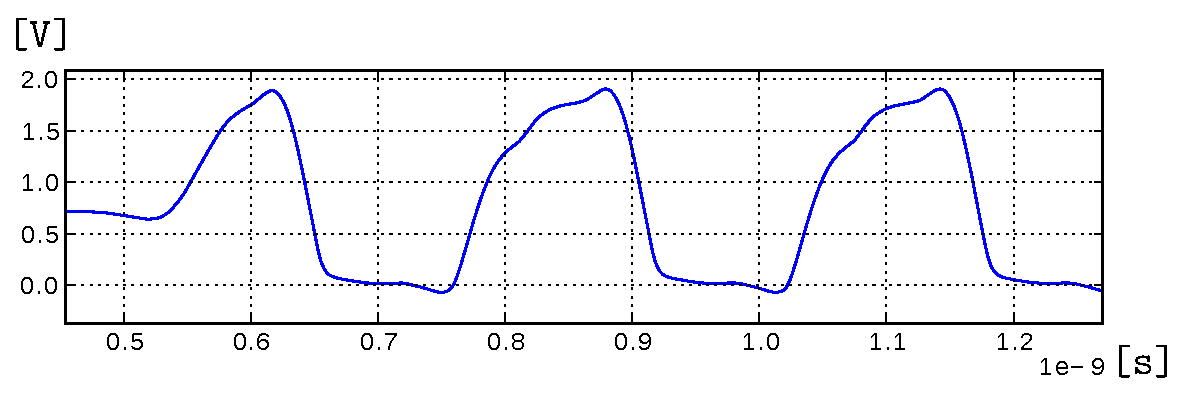
\includegraphics[scale=.6]{figuras/RO5.eps}
%  \caption{Simulación con parásitos extraidos del layout de la figura \ref{fig:RO5_lay}}
%\label{fig:RO5_wf}
%\vspace{-10pt}
%\end{figure}



%Para simular corners: opConditions.lib

%https://sites.google.com/site/cecstdcell/
%http://www.vlsitechnology.org/

